\section{Aim}
 To study PLpg/SQL triggers and exception handling.

\section{{Theory}}

\subsection{Triggers}

PostgreSQL Triggers are database callback functions, which are automatically performed/invoked when a specified database event occurs.

A trigger can be specified to fire when:
\begin{itemize}
	\item Before an INSERT, UPDATE, or DELETE operation
	\item After an INSERT, UPDATE, or DELETE operation
\end{itemize}

A trigger can be fired once for each table or once for each row.

A WHEN clause can be used to apply the trigger to specific rows only.

\subsubsection{Syntax}

\begin{minted}{sql}
CREATE  TRIGGER trigger_name [BEFORE|AFTER|INSTEAD OF] [INSERT|UPDATE|DELETE]
ON table_name
[
 -- Trigger logic goes here....
];
\end{minted}

\subsection{Exceptions}

By default, any exception that occurs during a transaction will abort the transaction. Exception handling can be implemented to properly handle the exception.

\subsubsection{Syntax}

\begin{minted}{sql}
RAISE EXCEPTION '[EXCEPTION]';
\end{minted}

\section{{Code and Output}}

\subsubsection{Create a table customer\_details (cust\_id (unique), cust\_name, address).\newline
Create a table emp\_details(empid(unique), empname, salary).\newline
Create table cust\_count(count\_row).\newline
}
\begin{enumerate}
\item Create a trigger whenever a new record is inserted in the customer\_details table.
\begin{minted}{sql}

CREATE OR REPLACE FUNCTION log_last_name_changes()
RETURNS trigger AS
$$
BEGIN
RAISE NOTICE 'A new row was inserted';
RETURN NEW;
END;
$$ LANGUAGE plpgsql;

CREATE TRIGGER last_name_changes
BEFORE INSERT
ON customer_details
FOR EACH ROW
EXECUTE PROCEDURE log_last_name_changes();
\end{minted}

\newline
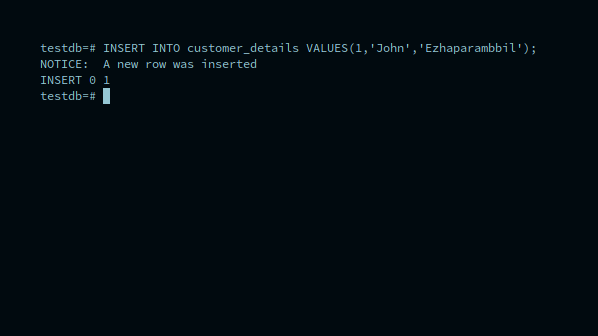
\includegraphics[width=\linewidth]{../Images/Triggers/1.png}

\item Create a trigger to display a message when a user enters a value greater than 20000 in the salary field of emp\_details table.
\begin{minted}{sql}

CREATE OR REPLACE FUNCTION log_sal_changes()
RETURNS trigger AS
$$
BEGIN
IF NEW.salary > 20000 THEN
RAISE NOTICE 'Employee has salary greater than 20000/-';
END IF;
RETURN NEW;
END;
$$ LANGUAGE plpgsql;

CREATE TRIGGER salary_changes
BEFORE INSERT
ON emp_details
FOR EACH ROW
EXECUTE PROCEDURE log_sal_changes();


\end{minted}

\newline
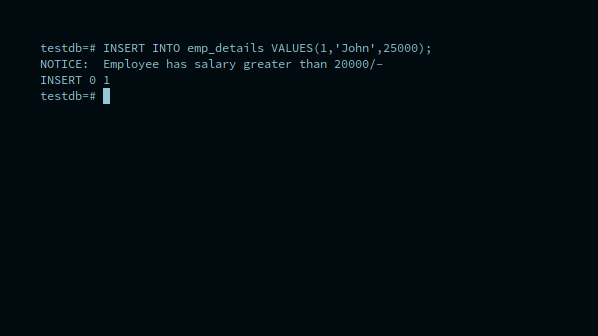
\includegraphics[width=\linewidth]{../Images/Triggers/2.png}

\item Create a trigger w.r.t customer\_detailstable.Increment the value of count\_row (in cust\_count table) whenever a new tuple is inserted and decrement the value of count\_row when a tuple is deleted. Initial value of the count\_row is set to 0.
\begin{minted}{sql}

CREATE OR REPLACE FUNCTION update_count()
RETURNS trigger AS
$$
BEGIN
UPDATE cust_count SET count_row = 
	(SELECT count(*) FROM customer_details);
RETURN NEW;
END;
$$ LANGUAGE plpgsql;

CREATE TRIGGER count_changes
AFTER INSERT OR DELETE
ON customer_details
FOR EACH ROW
EXECUTE PROCEDURE update_count();

\end{minted}

\newline
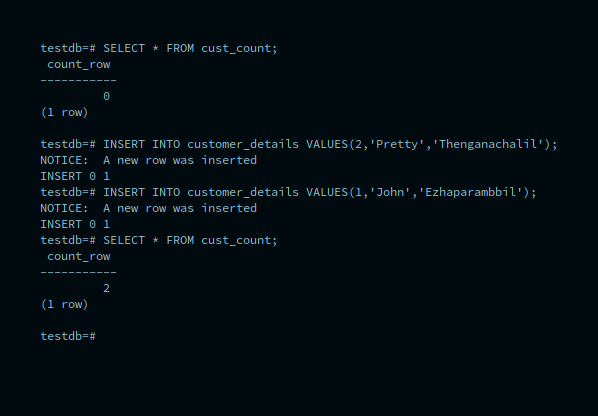
\includegraphics[width=\linewidth]{../Images/Triggers/3.png}

\newline
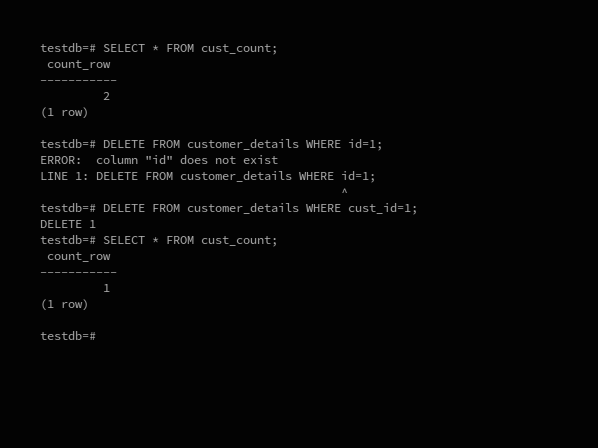
\includegraphics[width=\linewidth]{../Images/Triggers/8.png}

\item Create a trigger to insert the deleted rows from emp\_details to another table and updated rows to another table.(Create the tables deleted and updated)
\begin{minted}{sql}
CREATE OR REPLACE FUNCTION archive_deleted()
RETURNS trigger AS
$$
BEGIN
INSERT INTO deleted VALUES(OLD.*);
RETURN NEW;
END;
$$ LANGUAGE plpgsql;

CREATE OR REPLACE FUNCTION archive_updated()
RETURNS trigger AS
$$
BEGIN
INSERT INTO updated VALUES(OLD.*);
RETURN NEW;
END;
$$ LANGUAGE plpgsql;

CREATE TRIGGER archive_deleted_trig
BEFORE DELETE
ON emp_details
FOR EACH ROW
EXECUTE PROCEDURE archive_deleted();

CREATE TRIGGER archive_updated_trig
BEFORE UPDATE
ON emp_details
FOR EACH ROW
EXECUTE PROCEDURE archive_updated();

\end{minted}

\newline
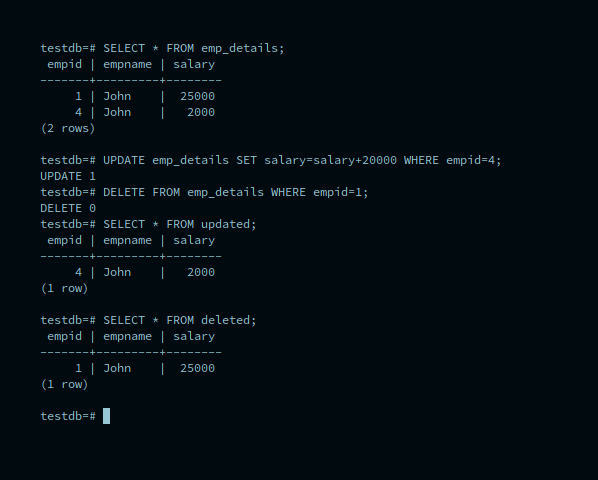
\includegraphics[width=\linewidth]{../Images/Triggers/4.png}

\item Write a PL/SQL to show divide by zero exception
\begin{minted}{sql}
CREATE OR REPLACE FUNCTION divide(a REAL, b REAL)
RETURNS REAL AS
$$
BEGIN
IF b = 0 THEN
RAISE EXCEPTION 'Division by Zero';
RETURN null;
ELSE
RETURN a / b;
END IF;
END;
$$ LANGUAGE plpgsql;

\end{minted}

\newline
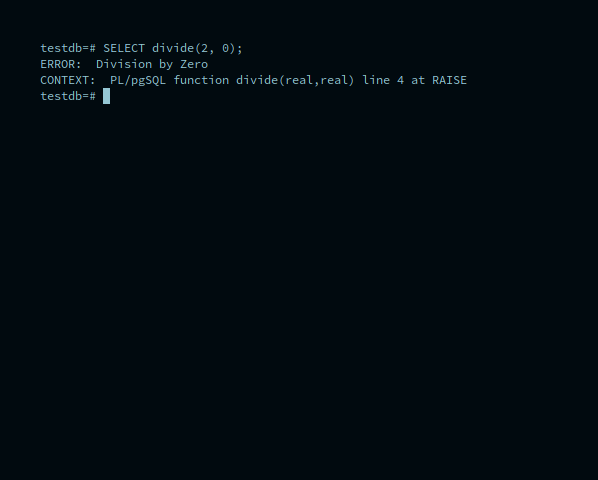
\includegraphics[width=\linewidth]{../Images/Triggers/5.png}

\item Write a PL/SQL to show no data found exception
\begin{minted}{sql}
CREATE OR REPLACE FUNCTION func_ex() RETURNS trigger AS
$$
DECLARE
var_name name;
BEGIN
WHEN NO_DATA_FOUND THEN 
	RAISE EXCEPTION 'No data found. Try another query.';
RETURN NEW;
END;
$$ LANGUAGE plpgsql;
CREATE TRIGGER insert_trigger AFTER UPDATE ON 
	people_list EXECUTE PROCEDURE func_ex();

\end{minted}

\newline
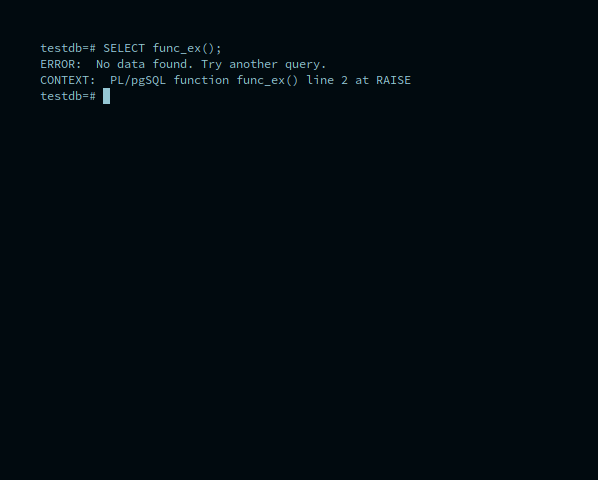
\includegraphics[width=\linewidth]{../Images/Triggers/6.png}


\item Create a table with ebill(cname,prevreading,currreading). If prevreading = currreading then raise an exception ‘Data Entry Error’.
\begin{minted}{sql}
CREATE OR REPLACE FUNCTION check_bill()
RETURNS TRIGGER AS
$$
BEGIN
IF NEW.prevreading = NEW.currreading THEN
RAISE EXCEPTION 'Data Entry Error';
RETURN OLD;
ELSE
RETURN NEW;
END IF;
END;
$$ LANGUAGE plpgsql;

CREATE TRIGGER bill_check
BEFORE INSERT
ON ebill
FOR EACH ROW
EXECUTE PROCEDURE check_bill();

\end{minted}


\newline
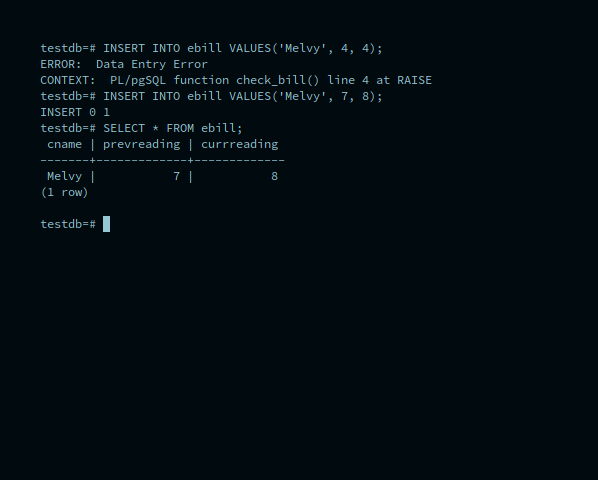
\includegraphics[width=\linewidth]{../Images/Triggers/7.png}
\end{enumerate}

\section{Result}
Implemented the program for Triggers and Exception Handling using Postgresql 11.5 on Manjaro Linux and the output was obtained.